\chapter{Introduction}
\label{sec:intro}
\acresetall
\acp{MAV} are an emerging technology that support society in a wide range of consumer, industrial and safety applications. For example \acp{MAV} are used to deliver medicine\cite{Shankland2018}, fight fires \cite{KateBaggaley2017} or even find survivors in disaster situations \cite{JoshuaBateman2017}.

\begin{figure}[b]
	\centering
	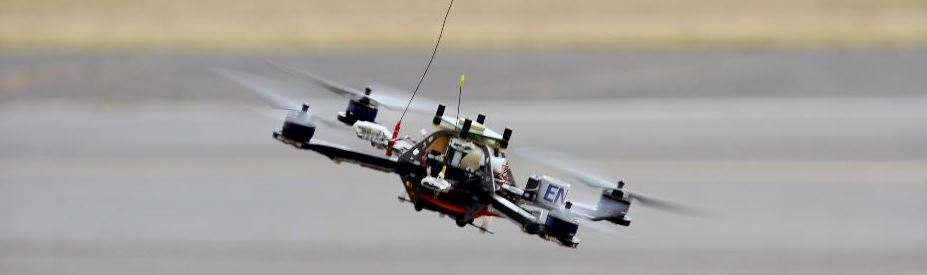
\includegraphics[width=\textwidth]{fig/mav}
	\caption{An example of Quadrotor-\ac{MAV}-Platform how it used in this thesis.}
	\label{fig:mav}
\end{figure}

Especially in emergency scenarios the fast and safe flight of \acp{MAV} is crucial to deliver help quickly and save human lives. However, due to the complexity of such missions as well as the difficulty to control an \ac{MAV} in these kind of scenarios, often multiple human operators are required in order to ensure safe operation \cite{Murphy2016}. With humans in the loop a constant connection between the \ac{MAV} and the operators is required which not only uses energy and requires infrastructure but also significantly reduces the reaction time. Enabling \acp{MAV} to fly more autonomously could allow less human operators to control more \acp{MAV} and thus to improve the support in emergency situations.

A major challenge on the way to the full autonomous flight of \acp{MAV} is the accurate estimation of the \ac{MAV}'s state within its environment. The system is highly dynamic so position and orientation can change rapidly. At the same time noise introduced by motor vibrations makes the position estimation with on-board \acp{IMU} alone too inaccurate \cite{Mohamed2014}. \ac{LIDAR}-sensors can capture long and wide range 3D information but the sensors are typically heavy and require energy. \ac{IR} sensors can cover distance information but are often limited in their \ac{FoV} as well as their range. External infrastructure like \ac{GPS} and optical tracking systems can provide accurate measurements but there is no guarantee that such systems are present in real world applications. Cameras on the other hand are cheap, lightweight and can measure long range distance information. This makes them a suitable choice as a sensor for on-board state estimation on light \acp{MAV} \cite{Elbanhawi2017}.

However, the signal delivered by the camera is high dimensional data that can not directly be interpreted as position or orientation measurement. Further processing by Computer Vision algorithms is required to interpret the image and extract relevant information. Thereby Machine Learning based methods are a popular choice to process the signal. Instead of designing an algorithm manually, the image processing is learned by using annotated examples. In particular Deep Learning based methods aim to combine whole Computer Vision pipelines into one mapping that transforms the raw input image into task dependent output. Experiments have shown how Deep Learning based methods outperform traditional Machine Learning approaches and manually crafted algorithms in a lot of examples \cite{Razavian}. This made them predominant choice for almost any vision task.

The hereby used \acp{CNN} are designed in a hierarchical way, using multiple layers that are evaluated sequentially. An example architecture is displayed in \Cref{fig:cnn_example}. By stacking more layers on top of each other (deepening) and increasing the number of nodes per layer (widening), highly non-linear functions can be modelled. Various experiments have shown the superior performance of particularly deep/wide models \cite{He, He2015, Szegedy2014, Zagoruyko2016}. However, this model flexibility assumed to be the reason for their superior performance also leads to immense requirements in computational resources. For example a state-of-the-art Computer Vision model \cite{He2015} contains 60.2 million parameters and one inference requires 11.3 billion floating point operations \cite{Tschannen2017}. 

\begin{figure}[bhtp]
	\centering
	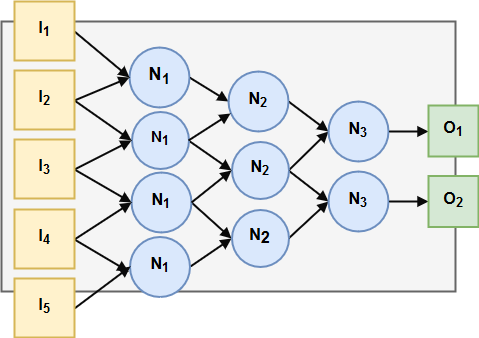
\includegraphics[width=0.5\textwidth]{fig/cnn_example}
	\caption{Simple Example Architecture of a \ac{CNN} with three layers. The input image $I$ is transformed by the nodes $N$ to the desired output $O$. Thereby each node represents a non-linear transformation of its inputs. The transformations are applied locally so the early layers perform operations on small patches of the image. Later stage combine this output hierarchically until the final output is reached. The parameters of each node are learned from annotated examples.}
	\label{fig:cnn_example}
\end{figure}

On robotic platforms like \acp{MAV} that have limited resources in terms of processing power and battery life but need to follow real-time constraints the deployment of such methods is still an open challenge. Despite a lot of research that addresses to reduce the number of computations in Deep Learning models \cite{YoungwanLee, Zagoruyko2016, Howard2017, Ghosh2017, Sandler2018, Zhang2017a} the investigation of relatively shallow models with less than ten layers received only little attention by the research community.

This work investigates the deployment of a Deep Learning based Computer Vision pipeline on a \ac{MAV}. The method is applied in the challenging scenario of Autonomous Drone Racing at the \ac{IROS} 2018. Within the race court several metal gates are placed and need to be passed one after another. Detecting the gates, allows to estimate the \ac{MAV}'s relative position and to calculate the flying trajectory. An overview of the race court and the racing gates at the \ac{IROS} 2016 Autonomous Drone Race can be seen in \Cref{fig:race_court}.

\begin{figure}[bhtp]
	\centering
	\begin{minipage}{0.45\linewidth}
	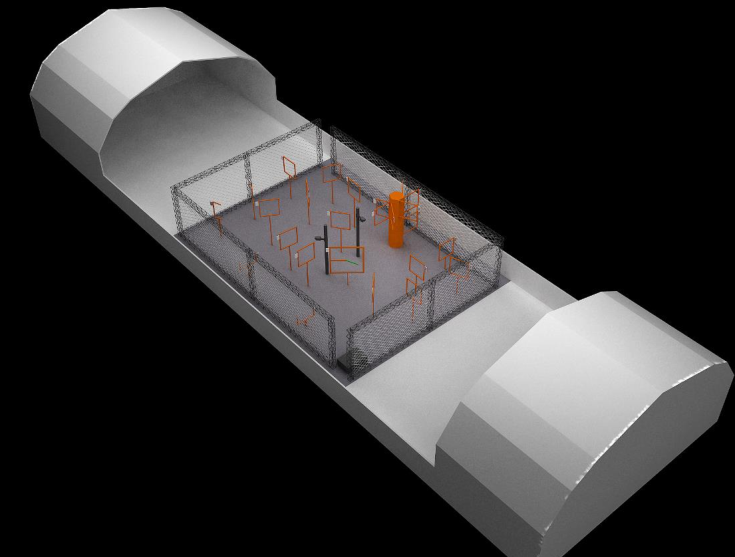
\includegraphics[width=\textwidth]{fig/race_court}
	\end{minipage}\hfill
\begin{minipage}{0.45\linewidth}
	\includegraphics[width=\textwidth]{fig/race_court_side}
\end{minipage}
\caption{Example Images of the \ac{IROS} 2016 Autonomous Drone Race}
\label{fig:race_court}
\end{figure}

The thesis builds on previous work by Ozo et. al \todoref{Reference to Current Method once it is published} which uses a manually crafted image processing method to detect the racing gates. Although fast to execute the method is very sensitive to illumination changes. Moreover, the algorithm fails when the objects are too far away or the frame is very thin. In order to develop a more robust method, this thesis investigates a learning based approach to the detection of racing gates.

In contrast to a lot of objects in the real world that are made of distinct and complex shapes like a pedestrian that consists of body parts and a face, the racing gates contain only thin edges and corners that are spread over large distances in the image. Additionally a majority of the area covered by the object is transparent and can therefore contain all kind of shapes, including other gates that stand behind the object. This introduces a particular vision task that even humans have a hard time at solving \footnote{The unconvinced reader can try to count the number of gates visible in the right image of \Cref{fig:race_court}} and that affects the training and design of a Computer Vision pipeline that aims to detect these kind of objects.

This thesis defines the class of objects as \textbf{\ac{EWFO}} and methods for their detection are studied in two examples which can be seen in \Cref{fig:gates} \todo{replace this with nicer images}. To the best of the authors knowledge \ac{EWFO} have not been particularly addressed in Computer Vision. In \cite{Falanga} and \cite{Li2018a} the authors also detect racing gates, however the used objects contain more structure than the ones investigated in this thesis. \citeauthor{Jung2018} present a framework to detect similar objects in \cite{Jung} and \cite{Jung2018} but they don't study the particular effects of to the object shape. \Cref{sec:object_detection} particularly addresses the implications of the object shape in modelling a Deep Learning based detection system for \ac{EWFO}.

A drawback of Deep Learning based vision systems is their need for vast amounts of annotated examples, which is not available for many applications. Racing gates for example are not an object that appears often in everyday life and therefore not many example images exist. To this end no publicly available dataset can be used to train a Computer Vision system for \ac{EWFO}. Since the object is transparent, it is particularly crucial that the training set covers a large variety of backgrounds. Otherwise, it is likely that a model uses the background for prediction and only works in a particular domain. Although building a race court, placing it in a large variety of scenes and annotating taken images is theoretically possible, it is a cumbersome and very time consuming task. 

\begin{figure}[bhtp]
	\centering
	\begin{minipage}{0.45\linewidth}
		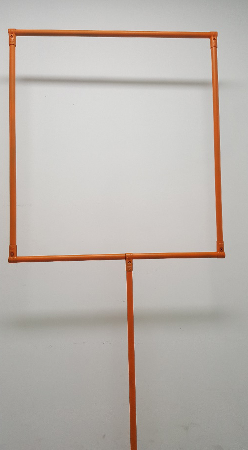
\includegraphics[height=5cm]{fig/gate1}
	\end{minipage}\hfill
	\begin{minipage}{0.45\linewidth}
		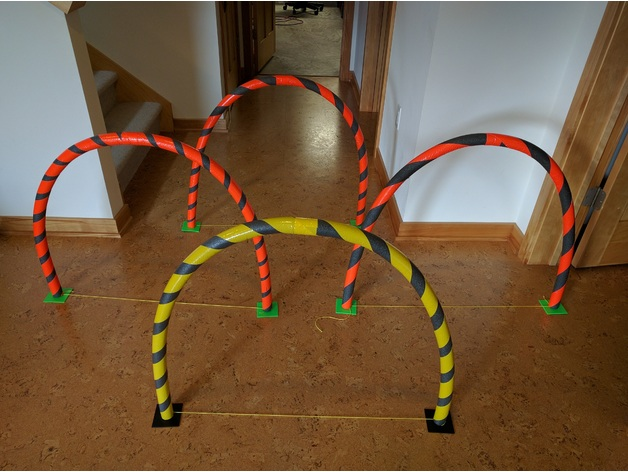
\includegraphics[width=\textwidth]{fig/gate2}
	\end{minipage}
	\caption{Example Images of the Empty Wire Frame Objects investigated in this thesis. }
	\label{fig:gates}
\end{figure}

Moreover, the view of a \ac{FPV} camera mounted on an \ac{MAV} can be substantially different from a normal camera as well as between different \ac{MAV}-platforms. For example the often used wide-angle lenses, used to increase the \ac{FoV} of the visual sensor, lead to image distortion that changes the appearance of objects and scene. A Machine Learning based vision system needs to take these implications into account when selecting the training data. 

Alternatively to annotating real images the training data can be synthesized using graphical engines. This not only allows the rendering of a large amount of backgrounds it also enables the theoretically infinite generation of training data. Moreover, it allows to model and incorporate domain specific properties like lens distortion or motion blur into the training process. However, a graphical engine can never fully model the real world which needs to be considered when generating synthetic data. \Cref{sec:training} studies the generation of artificial data to train an object detector for \ac{EWFO}.

Without an accurate detection of the racing gate, the \ac{MAV} is not able to determine its current position and thus to calculate its flying trajectory. On the other hand, with a algorithm that requires less computational resources a lighter \ac{MAV} can be built. This allows faster and more aggressive trajectories as well as longer battery live. Hence, the trade-off between accuracy and inference speed is of particular interest for this application and is addressed in \Cref{sec:tradeoff}.

\section{Research Question}

This section summarizes the research question addressed in this thesis. Furthermore it describes how the question is split in multiple subquestions that are addressed in the individual chapters.

	\textbf{How can the detection of wire frame objects on an \ac{MAV} with resource and time constraints, be modelled and learned from synthetic data?}


\begin{enumerate}
	\item[\textbf{RQ1}]How can data be generated to train a detection model for \ac{EWFO} detection on a \acp{MAV}?
	\item[\textbf{RQ2}]How can a detection model represent \acp{EWFO}?
	\item[\textbf{RQ3}]What are the trade-offs in detection performance and inference time when a detection model for \acp{EWFO} is deployed on a \ac{MAV}?
	\item[\textbf{RQ4}]Can the gained insights be used to build a lightweight and robust detection model for racing gates in the \ac{IROS} Autonomous Drone Race?
\end{enumerate}

\section{Results/Contributions}

\todo{Put some results at the end.}

\section{Outline}

The thesis is structured as follows: \Cref{sec:evaluation} describes the metrics and systems used for evaluation. \Cref{sec:training}, \Cref{sec:object_detection},\Cref{sec:tradeoff} and \Cref{sec:method} address the individual research questions. Each chapter contains an introduction to the topic, the methodology used in this thesis and experiments that have been carried out. \Cref{sec:training} describes methods to generate synthetic data for machine learning. It concludes with the datasets used for the remaining parts of this thesis.  \Cref{sec:object_detection} describes object detection and evaluates current methods in the application for wire frame objects. \Cref{sec:tradeoff} illustrates and evaluates measures to reduce computations and optimize an object detection system for a particular hardware. It investigates the trade-off between detection performance and inference time. \Cref{sec:method} describes how the gained insights are used to develop a detector for racing gates at the \ac{IROS} 2018 Autonomous Drone Race. It also compares the current method to a traditional image processing method in terms of speed and detection performance. \Cref{sec:disc} discusses the overall results and formulates a conclusion.
